\documentclass[journal]{IEEEtran}

% --- Required packages ---
\usepackage[utf8]{inputenc}
\usepackage[T1]{fontenc}
\usepackage[english]{babel}
\usepackage{cite}
\usepackage{amsmath,amssymb,amsfonts}

\usepackage{graphicx}
\graphicspath{{figfinals/}}

\usepackage{caption}
\usepackage{subcaption}

\usepackage{colortbl}
\usepackage{textcomp}
\usepackage{xcolor}
\usepackage[hyphens]{url}
\usepackage{booktabs}
\usepackage{multirow}
\usepackage{array}
\usepackage{threeparttable}
\usepackage{siunitx}

\begin{document}
	
	% ---------------------------------------------------------------
	% TITLE AND AUTHORSHIP
	% ---------------------------------------------------------------
	\title{UniVoice: Breaking Communication Barriers Through AI-Powered Multimodal Messaging for Users with Sensory Impairments}
	
	\author{Gleiston~Guerrero-Ulloa,%
		Jhon~B.~Leturne-Pluas,%
		Miguel~J.~Hornos,%
		and~Carlos~Rodr\'iguez-Dom\'inguez%
		\thanks{Manuscript received XX Month 2026; revised XX Month 2026;
			accepted XX Month 2026. Date of publication XX Month 2026;
			date of current version XX Month 2026.
			This work was supported by institutional resources of the
			Universidad T\'ecnica Estatal de Quevedo (UTEQ) and the
			Universidad de Granada (UGR).
			\textit{(Corresponding author: Gleiston Guerrero-Ulloa.)}}%
		\thanks{G.~Guerrero-Ulloa and J.~B.~Leturne-Pluas are with the
			Faculty of Computer Sciences, Universidad T\'ecnica Estatal de
			Quevedo, Quevedo 120501, Los R\'ios, Ecuador (e-mail:
			gguerrero@uteq.edu.ec; jleturnep@uteq.edu.ec).}%
		\thanks{M.~J.~Hornos and C.~Rodr\'iguez-Dom\'inguez are with the
			Department of Software Engineering, Universidad de Granada,
			18071 Granada, Spain (e-mail: mhornos@ugr.es;
			carlosrodriguez@ugr.es).}%
		\thanks{Color versions of one or more figures in this article are
			available at \protect\url{https://doi.org/10.1109/JIOT.2026.xxxxxxx}.}%
		\thanks{Digital Object Identifier~10.1109/JIOT.2026.xxxxxxx}}
	
	\markboth{IEEE Internet of Things Journal,~Vol.~XX, No.~X, 2026}%
	{Guerrero-Ulloa~\MakeLowercase{\textit{et al.}}:
		UniVoice --- AI-Powered Inclusive Mobile Messaging}
	
	\maketitle
	
	% ---------------------------------------------------------------
	% ABSTRACT
	% ---------------------------------------------------------------
	\begin{abstract}
		The digital exclusion of people with sensory disabilities from mobile
		messaging platforms represents one of the most pressing challenges in
		human-centred software engineering.
		This article presents the design, implementation, and empirical
		evaluation of \textsf{UniVoice}, an AI-powered inclusive mobile
		messaging system conceived for users with visual, hearing, and
		speech disabilities. For users with visual impairment, the system provides
		text-to-speech~(TTS), voice command navigation, automatic image
		description~(OCR\,+\,BLIP captioning), and audio transcription.
		For users with hearing impairment, the system provides
		speech-to-text~(STT) transcription of received audio and video.
		For users with speech disability---which clinically decomposes into the
		deaf-mute subgroup and the speech-only-impairment subgroup---coverage is
		established through the receiver-adaptation logic of \textsf{UniVoice}
		without a dedicated AAC module: deaf-mute users are served by the union
		of the hearing-impairment adaptations (STT of received audio) and
		text-based composition for sending, and speech-only-impaired users retain
		full reception of every modality while composing messages via the mobile
		touchscreen, with recipient-dependent TTS when the addressee has a visual
		impairment.
		The proposed architecture integrates an intelligent processing API
		that orchestrates TTS, STT, automatic image description via computer
		vision, and optical character recognition~(OCR) modules, dynamically
		adapting each message format to the receiver's sensory profile.
		The technology stack combines React~Native for a cross-platform mobile
		interface, Spring~Boot~(Java) for business logic, Django~(Python) for
		AI processing, RabbitMQ as a message broker, and PostgreSQL for
		persistence, with end-to-end asymmetric-key encryption.
		Development followed the TDDM4IoTS methodology
		(\textit{Test-Driven Development Methodology for IoT-Based Systems}).
		\textsf{UniVoice} was evaluated with $n{=}25$ participants (60\,\% with visual impairment, 20\,\% with hearing impairment, and 20\,\% without disability) applying the Technology Acceptance Model~(TAM) and a WCAG~2.1 checklist. Results revealed a global TAM mean of $\bar{x}{=}4.20$/5 ($\bar{x}_{\text{PU}}{=}4.55$; $\bar{x}_{\text{PEOU}}{=}3.85$), strong internal consistency ($\alpha{=}0.866$; PU: $\alpha{=}0.867$; PEOU: $\alpha{=}0.898$), and the highest-rated item reaching 84\,\% maximum-scale responses. An iterative accessibility improvement cycle produced a 64\,\%
		reduction in WCAG~2.1 warnings. The findings validate that strategic AI integration in mobile applications constitutes a viable approach to bridging the communicative gap of people with sensory disabilities.
	\end{abstract}
	
	\begin{IEEEkeywords}
		Accessibility, assistive technology, end-to-end encryption,
		human-machine interaction, image captioning, inclusive messaging,
		mobile application, React~Native, sensory disability, speech
		recognition, speech synthesis, TAM, TDDM4IoTS, UniVoice, WCAG.
	\end{IEEEkeywords}
	
	% ---------------------------------------------------------------
	% I. INTRODUCTION
	% ---------------------------------------------------------------
	\section{Introduction}
	\label{sec:intro}
	\IEEEPARstart{I}{nstantaneous} communication has become a fundamental right in contemporary society and a cornerstone of full civic participation. Despite mobile messaging platforms surpassing three billion active users globally, their proliferation has not been matched by intrinsic accessibility architectures that guarantee equitable use for individuals with sensory impairments.
	
	The scale of the population affected is global. The World Health Organization~(WHO) estimates that approximately $15\,\%$ of the world population lives with some form of disability~\cite{who2011}, a proportion of which concerns the three sensory profiles targeted by this work. For hearing impairment, the WHO reports that over $5\,\%$ of the world's population---some 430 million people, projected to exceed 700 million by 2050---require rehabilitation for disabling hearing loss~\cite{who2021hearing}. For visual impairment, at least 2.2 billion people live with near- or distance-vision impairment worldwide, of whom at least one billion face a condition that could have been prevented or remains unaddressed~\cite{who2023vision}. For speech, voice, and language disorders, population data from national surveillance systems range from $7.7\,\%$ prevalence among U.S.\ children aged 3--17~\cite{nidcd2024} to 40 million Americans with a communication disorder of some form~\cite{asha2023}. At the regional level, the Pan American Health Organization estimates that 217 million people in the Region of the Americas live with hearing loss ($21.52\,\%$ of the regional population), with a projected rise to 322 million by 2050~\cite{paho2023hearing}. Within this regional frame, Ecuador's National Council for Disability Equality~(CONADIS) registers 124{,}801 individuals with active sensory disabilities, distributed as $50.30\,\%$ hearing, $45.39\,\%$ visual, and $4.31\,\%$ speech impairments, with 70{,}429 men~($56.4\,\%$) and 54{,}372 women~($43.6\,\%$)~\cite{conadis2024}. The Ecuadorian figures illustrate at a national scale the structural patterns---hearing dominant over visual, speech a smaller but non-negligible tail---consistent with the global and regional estimates.
	
	The most widely used messaging platforms---WhatsApp, Telegram, Messenger, and Instagram---offer only partial accessibility features: limited screen-reader compatibility (TalkBack and VoiceOver), contrast adjustment, and, in the case of WhatsApp, recently introduced audio-to-text transcription. However, none of these platforms comprehensively addresses the needs of users with multiple sensory profiles: bidirectional adaptation among text, audio, and image modalities; automatic semantic description of visual content; complete navigation by voice commands; nor end-to-end encryption for accessible multimodal data flows~\cite{bercaru2024,weichbroth2020}.
	
	A third population---users with speech (verbal production) disabilities---requires a dedicated functional analysis because ``speech disability'' is not a homogeneous clinical category. Standard clinical taxonomies~\cite{elsahar2019,bleakley2022,costanzo2023} distinguish two functionally distinct subgroups on the basis of the auditory-channel status. The first subgroup comprises \emph{deaf-mute users} (pre-lingual profound hearing loss in which oral speech has not developed or is not functional for communication), whose auditory and speech channels are simultaneously impaired~\cite{saleem2023,kothadiya2022}. The second subgroup comprises users with \emph{speech-only impairment}---dysarthria, aphasia, selective mutism, post-laryngectomy aphonia, or severe stammering---whose hearing and vision remain intact and whose only functional barrier is the production of voice.
	
	Within the receiver-adaptation logic of \textsf{UniVoice}---the system proposed in this article---both subgroups are fully covered \emph{without} a dedicated AAC module. Deaf-mute users share the functional barriers of the hearing-impairment profile (inability to consume incoming audio without STT mediation) and those of the speech-impairment profile (inability to produce outgoing audio without text input); the hearing-impairment adaptations already implemented in \textsf{UniVoice}---STT transcription of received audio/video and text-based composition of outgoing messages---therefore fully cover this subgroup with no additional engineering. Users with speech-only impairment retain unimpeded reception of every message modality (text, audio, image, video), so their reception profile is identical to that of a non-disabled user; for sending, the mobile touchscreen provides text-based composition as a universally available, fully effective alternative to voice input, and when the recipient has a visual impairment, \textsf{UniVoice} applies TTS to the outgoing text to preserve communicative equivalence with a voice-capable sender. This two-subgroup argument establishes that the taxonomy of the speech-disability population does not introduce a third functional case beyond those already addressed by the hearing and non-disabled reception profiles, and justifies the absence of a dedicated AAC module in the present architecture. Enhanced input assistance for severe speech disorders~\cite{bleakley2022,costanzo2023}---personalised disfluency-tolerant STT, phrase banks, predictive text tailored to residual articulatory patterns---remains a complementary future-work priority rather than a gap in the current coverage claim.
	
	From a Human-Machine Interaction~(HMI) perspective, universal design~\cite{story1998} and the Web Content Accessibility Guidelines~(WCAG~2.1)~\cite{w3c2018} require that systems be perceivable, operable, understandable, and robust for the widest possible range of users. In the mobile context, systematic accessibility evaluations of Android and iOS applications reveal non-compliance rates exceeding $60\,\%$ in criteria such as text alternatives for non-text content and complete navigation without precise touch interaction~\cite{chen2022,acosta2021}. Against this background, recent advances in Artificial Intelligence~(AI) offer unprecedented opportunities to overcome these barriers: state-of-the-art deep neural network TTS systems produce naturalistic speech synthesis~\cite{tan2021}, transformer-based speech-to-text models have achieved word error rates~(WER) comparable to human transcription~\cite{baevski2020}, and image captioning models have demonstrated practical utility for users with visual disabilities in real-world scenarios~\cite{dognin2021}.
	
	The present work is motivated by the following research questions:
	\begin{itemize}
		\item[\textbf{RQ1}] Can a single mobile platform coherently integrate TTS, STT, image captioning, and OCR modules---together with asymmetric end-to-end encryption---while maintaining zero processing error rates under variable input conditions?
		\item[\textbf{RQ2}] Does the proposed system achieve a Technology Acceptance Model score above the positive acceptance threshold of $\bar{x}{>}4.0$ in a heterogeneous population of individuals with sensory disabilities?
		\item[\textbf{RQ3}] Can the TDDM4IoTS development methodology, applied with accessibility as a formal acceptance criterion, produce a measurable and statistically meaningful reduction in WCAG~2.1 warnings compared to leading commercial messaging platforms?
	\end{itemize}
	
	The contributions of this work are: (\textit{i})~an accessibility-oriented microservices architecture that integrates TTS, STT, OCR, image description, and asymmetric end-to-end encryption in a cross-platform mobile messaging system (addressing~RQ1); (\textit{ii})~a systematic application of the TDDM4IoTS methodology~\cite{guerrero2020} to inclusive messaging software development; (\textit{iii})~empirical evidence on technological acceptance---measured via TAM---and technical accessibility from a study involving 25 participants with heterogeneous sensory disabilities (addressing~RQ2); and (\textit{iv})~quantification of the impact of an iterative accessibility improvement process, achieving a global $64\,\%$ reduction in warnings identified by Google's Accessibility Scanner (addressing~RQ3).
	
	The remainder of this article is organised as follows. Section~\ref{sec:related} reviews related work along three dimensions: accessibility in mobile messaging, augmentative and alternative communication~(AAC), and AI for accessibility, identifying the gaps that motivate this research. Section~\ref{sec:methodology} describes the mixed-methods research paradigm, the eleven TDDM4IoTS phases applied---including the microservices architecture, intelligent message-conversion flow, voice-command module, asymmetric encryption, and hybrid infrastructure---and the 18 WCAG~2.1 accessibility criteria employed. Section~\ref{sec:evaluation} presents technical API performance results (TTS, STT, image description, video), iterative accessibility results, and TAM questionnaire results. Section~\ref{sec:discussion} interprets the findings in the context of existing literature and reflects on the implications for the Sustainable Development Goals. Section~\ref{sec:conclusion} synthesises the main conclusions and directions for future research.
	
	% ---------------------------------------------------------------
	% II. RELATED WORK
	% ---------------------------------------------------------------
	\section{Related Work}
	\label{sec:related}
	
	\subsection{Accessibility in Mobile Messaging Applications}
	
	\subsubsection{Empirical evaluations with real users}
	Weichbroth \cite{weichbroth2020} conducted a systematic review of
	57 usability studies on mobile applications, concluding that
	accessibility is among the least addressed criteria in conventional
	design processes.
	Chen~\textit{et al.} \cite{chen2022} carried out a large-scale
	empirical study of Android app accessibility---including popular
	messaging platforms---revealing non-compliance rates exceeding
	60\,\% in fundamental WCAG~2.1 criteria such as text alternatives
	for non-text content, semantic labelling, and screen-reader
	compatibility.
	
	Da~Silva~\textit{et al.} \cite{dasilva2016} performed the first
	systematic evaluation of WhatsApp from the perspective of visually
	impaired users, identifying 18 critical barriers including
	absent alternative texts, insufficient auditory feedback on
	notifications, and low visibility of interactive control states.
	Zahida~\textit{et al.} \cite{zahida2021} extended this approach
	to elderly users, documenting that absent persistent font-size
	adjustment, icon density on small screens, and insufficient
	haptic feedback are primary error sources.
	Swati~\textit{et al.} \cite{swati2021} found that Facebook
	Messenger is systematically inaccessible for users with complete
	blindness due to missing accessibility labels on critical buttons.
	Rumini and Astrid \cite{rumini2019} identified that aesthetic and
	consistency dimensions present the greatest violations in
	Telegram according to Nielsen's heuristics.
	Kim~\textit{et al.} \cite{kim2024} found significant deficiencies
	in the emotional and affective interface design of mobile
	communication apps for hearing-impaired users.
	
	\subsubsection{Systematic reviews and accessibility frameworks}
	Ballantyne~\textit{et al.} \cite{ballantyne2018} compared W3C,
	Google, Apple, and other normative accessibility guidelines,
	concluding that cross-platform fragmentation creates inconsistencies
	and recommending WCAG~2.1 as the transversal reference.
	Acosta-Vargas~\textit{et al.} \cite{acosta2021} demonstrated that
	a combined automated-plus-manual approach increases detection
	coverage by more than 35\,\%.
	Huang~\textit{et al.} \cite{huang2025} evaluated the four most
	widely used messaging platforms with adults with mild-to-moderate
	cognitive disabilities, documenting systematic failures in
	touch-target size, colour contrast, and screen orientation.
	Bercaru and Popescu \cite{bercaru2024} conducted a PRISMA review of
	2{,}819 articles concluding that adaptive personalisation of user
	experience remains the most deficient dimension in accessibility
	research.
	
	\subsection{Augmentative and Alternative Communication Systems}
	
	\subsubsection{Conceptual framework and base technologies}
	Elsahar~\textit{et al.} \cite{elsahar2019} systematised modalities
	of AAC high-technology platforms and concluded that machine learning
	represents the most promising avenue, particularly through speech
	generation, text prediction, and biological signal classification.
	Guerrero-Ulloa~\textit{et al.} \cite{guerrero2021bellchat}
	presented BellChat, the first inclusive web messaging application
	integrating simultaneous TTS and STT for users with visual
	and hearing disabilities, though limited to a web-only environment.
	Yeratziotis~\textit{et al.} \cite{yeratziotis2023} integrated
	sign language into social media apps for deaf users; however,
	their approach does not address visual disability or speech impairment.
	Chang~\textit{et al.} \cite{chang2022} proposed a smart city
	system combining gesture and voice recognition for hearing- and
	visually-impaired citizens.
	Janaka~\textit{et al.} \cite{janaka2023} explored ubiquitous
	messaging via smart glasses, demonstrating that voice input reduces
	response time by 33.1\,\% and increases typing speed by 40.3\,\%.
	
	\subsubsection{AI-based AAC applications for speech disorders}
	Costanzo~\textit{et al.} \cite{costanzo2023} evaluated Talkitt---an
	ML application that translates unintelligible sounds into clear
	words---with children with Down syndrome, showing recognition
	precision improved from 75\,\% to 90\,\% after personalised
	calibration.
	Mateos-Sanchez~\textit{et al.} \cite{mateos2022} developed
	CapacitaBOT, an IBM~Watson conversational chatbot for people
	with intellectual disabilities.
	Bleakley~\textit{et al.} \cite{bleakley2022} documented critical
	barriers in commercial STT systems for people who stammer:
	excessively short end-of-utterance detection windows and inability
	to manage disfluencies, with direct implications for inclusive
	STT module design.
	
	\subsection{Artificial Intelligence for Accessibility}
	
	Chemnad and Othman \cite{chemnad2024} conducted a PRISMA
	bibliometric review of 3{,}706 articles (2018--2023), presenting
	a classification framework for AI in accessibility and concluding
	that research is concentrated asymmetrically on visual
	disabilities while hearing, speech, cognitive, and motor
	disabilities receive significantly less coverage.
	Ji~\textit{et al.} \cite{ji2024} and Tan~\textit{et al.}
	\cite{tan2021} established the state of the art in neural TTS,
	while Baevski~\textit{et al.} \cite{baevski2020} and
	Radford~\textit{et al.} \cite{radford2023} demonstrated
	WER comparable to human transcription in STT systems.
	Ming~\textit{et al.} \cite{ming2022} published the most
	comprehensive review of automatic image captioning to date.
	Dognin~\textit{et al.} \cite{dognin2021} demonstrated on the
	VizWiz dataset---composed of images taken by blind people in
	real-world conditions---that modern captioning systems can reach
	utility levels comparable to human descriptions in accessibility
	contexts.
	Mukherjee~\textit{et al.} \cite{mukherjee2023} showed OCR
	accuracy exceeding 95\,\% for standard printed characters.
	Saleem~\textit{et al.} \cite{saleem2023},
	Papatsimouli~\textit{et al.} \cite{papatsimouli2023}, and
	Kothadiya~\textit{et al.} \cite{kothadiya2022} advanced
	real-time sign language recognition systems.
	
	\subsection{Identified Gaps}
	The critical analysis of the 35 reviewed works identifies five
	structural gaps that justify the contribution of this work.
	
	\textbf{Gap~1---Absence of multimodal mobile platforms simultaneously
		covering visual, hearing, and speech profiles.}
	No reviewed work implements a mobile messaging system that
	dynamically adapts each message to the receiver's sensory
	profile combining TTS, STT, image captioning, and OCR in a
	single native mobile platform.
	
	\textbf{Gap~2---Technological fragmentation:} mature AI components
	exist in isolation but have not been integrated in a coherent
	system with guaranteed privacy.
	No work combines TTS, STT, captioning, and OCR in a messaging
	architecture with asymmetric end-to-end encryption.
	
	\textbf{Gap~3---Scarcity of empirical TAM evidence} with
	heterogeneous multi-disability populations.
	Existing studies are restricted to single disability profiles.
	
	\textbf{Gap~4---Absence of systematic, test-driven development
		methodologies} for accessible messaging software.
	TDDM4IoTS has not previously been adapted to inclusive mobile
	messaging development.
	
	\textbf{Gap~5---Insufficient coverage of speech disorder profiles}
	in voice-input messaging systems.
	No existing system offers automatic input-mode adaptation
	according to the user's individual disfluency profile.
	
	This work directly addresses all five identified gaps.
	
	% ---------------------------------------------------------------
	% III. MATERIALS AND METHODS
	% ---------------------------------------------------------------
	\section{Materials and Methods}
	\label{sec:methodology}
	This section describes, first, the materials employed---platforms,
	instruments, and AI components---and, second, the methods applied
	for system development and for technical and user evaluation.
	The study adopted a mixed-methods research paradigm \cite{hernandez2014}:
	quantitative for API conversion performance metrics (mean latency,
	error rate) and for the TAM questionnaire; qualitative for the
	analysis of accessibility barriers identified during direct user
	observation sessions.
	The research type is applied and projective \cite{hernandez2014},
	oriented toward the design, implementation, and evaluation of a
	software artifact that solves a specific technical and social
	problem in inclusive communication.
	
	\subsection{Materials}
	
	\subsubsection{Hardware Infrastructure and Deployment}
	The system was deployed on a hybrid infrastructure consisting of two
	complementary nodes.
	The \textbf{AI node} is an Amazon Web Services~(AWS) instance
	running Windows~Server, assigned to the AI~API~(Django/Python)
	given its greater CPU and RAM demands for vision and language model
	inference.
	The \textbf{backend node} is a CentOS server administered by
	UTEQ, hosting the REST~API~(Spring~Boot/Java), the RabbitMQ
	message broker, and the PostgreSQL database.
	Nginx served as a web server and reverse proxy on both nodes;
	Docker containerization ensured portability and service isolation
	between development and production environments.
	Technical API tests were executed from an Android mobile device
	connected to a standard WiFi network (802.11n, $-$55\,dBm).
	
	\subsubsection{Technology Stack}
	Table~\ref{tab:stack} summarises the software components,
	selected technology, and technical justification for each choice.
	React~Native was selected for the mobile interface for its ability
	to generate native UI components for Android and iOS from a single
	codebase, reducing maintenance costs and ensuring compatibility
	with platform accessibility services (TalkBack on Android,
	VoiceOver on iOS).
	
	\begin{table}[!t]
		\caption{Technology Stack of the Inclusive Messaging System}
		\label{tab:stack}
		\centering
		\scriptsize
		\renewcommand{\arraystretch}{1.25}
		\begin{tabular}{p{1.8cm}p{1.8cm}p{3.3cm}}
			\toprule
			\textbf{Component} & \textbf{Technology} & \textbf{Justification} \\
			\midrule
			Mobile UI      & React Native   & Cross-platform; native TalkBack/VoiceOver support \\
			REST backend   & Spring Boot    & Microservices, ORM, horizontal scalability \\
			AI API         & Django (Python)& ML/NLP ecosystem, pre-trained models \\
			Real-time msg. & WebSocket + RabbitMQ & Ordered delivery, fault tolerance \\
			Persistence    & PostgreSQL     & Relational, ACID-compliant, open source \\
			Containers     & Docker + Nginx & Portability, isolation, reverse proxy \\
			Cloud (AI)     & AWS Windows Server & CPU/RAM for model inference \\
			Encryption     & Asymmetric keys & End-to-end confidentiality \\
			\bottomrule
		\end{tabular}
	\end{table}
	
	\subsubsection{Artificial Intelligence Components}
	The accessible conversion modules integrate the following AI
	components.
	For \textbf{TTS}, two engines were integrated in parallel:
	Edge-TTS~(Microsoft Neural TTS, multilingual, cloud-based)
	and SAPI5~(Microsoft Speech API~5, local processing via
	\texttt{pyttsx3}).
	For \textbf{STT}, a deep-learning transformer-based automatic
	speech recognition API~\cite{baevski2020,radford2023} was used
	(Whisper, executed on the AWS node).
	For \textbf{image description}, pre-trained
	vision-language models were integrated via API calls, specifically
	\texttt{blip-image-captioning-base} from Hugging~Face,
	consistent with the state of the art~\cite{dognin2021,safiya2024}.
	For \textbf{OCR}, computer vision models with accuracy exceeding
	95\,\% on standard printed text~\cite{mukherjee2023} were used.
	For \textbf{voice command navigation}, cosine
	similarity~\cite{lahitani2016} was used as a semantic proximity
	metric, with cascade correction via the Llama~1B language model
	and a phonetic dictionary.
	
	\subsubsection{Security and Privacy Threat Analysis}
	\label{sec:stride}
	The security architecture was analysed using the STRIDE threat
	modelling framework~\cite{shostack2014}, applied to the five
	principal communication flows documented in Fig.~\ref{fig:flujo}
	and Section~III-B2.
	Table~\ref{tab:stride} summarises threats, current mitigations,
	and residual gaps identified for each flow.
	
	The most critical finding concerns the \textbf{Information Disclosure}
	threat at the server-side conversion step~(F3): the Spring~Boot
	backend decrypts the message before forwarding it to Django,
	creating a transient plaintext window in server memory.
	The manuscript asserts that the server never stores plain text;
	however, no technical mechanism~(memory-scrubbing, trusted
	execution environment, or audit log) is documented to verify
	this assertion.
	This constitutes a transparency gap; its remediation via
	post-processing memory-scrubbing is designated as future work.
	
	\begin{table}[!t]
		\caption{STRIDE Threat Analysis of Principal Communication Flows.
			F1~=~registration; F2~=~client-to-server send;
			F3~=~server-side AI conversion; F4~=~server-to-receiver delivery;
			F5~=~key repository management.
			\checkmark~=~mitigated; $\triangle$~=~partial; $\times$~=~residual gap.}
		\label{tab:stride}
		\centering
		\scriptsize
		\renewcommand{\arraystretch}{1.25}
		\begin{tabular}{p{0.9cm}p{1.4cm}p{2.1cm}p{1.5cm}c}
			\toprule
			\textbf{Threat} & \textbf{Flow/asset} & \textbf{Scenario} & \textbf{Gap} & \textbf{St.} \\
			\midrule
			Spoofing & F1: Registration & Fake account, no identity check & No 2FA documented & $\triangle$ \\
			Tampering & F2/F4: WebSocket & Message modification in transit & No independent message signature & $\triangle$ \\
			Repudiation & F2: Sent msgs & Denial of authorship & No crypto non-repudiation & $\triangle$ \\
			Info. Discl. & F3: Conversion & Plaintext in server memory & No TEE or memory-scrub & $\times$ \\
			DoS & F3: Django API & Endpoint saturation & No rate limiting documented & $\triangle$ \\
			Elevation & F2: REST API & Privilege escalation & No RBAC analysis documented & $\times$ \\
			\bottomrule
		\end{tabular}
	\end{table}
	
	\subsubsection{Sensory Profile Coverage Model}
	\label{sec:coverage}
	Table~\ref{tab:coverage} presents the functional coverage matrix of \textsf{UniVoice} across four sensory profiles, with the speech-disability row resolved according to the two-subgroup taxonomy established in Section~\ref{sec:intro}. Users with \emph{speech-only impairment} retain intact auditory and visual function: reception coverage is therefore 100\,\% (audio messages are played directly, images are viewed directly, video is reproduced directly, and text is read visually), identical to the non-disabled reception profile. The sending channel relies on text-based composition as the primary input; when the recipient has a visual impairment, the system applies TTS conversion to the outgoing text, producing an audio message functionally equivalent to a voice-capable sender's output. Users with \emph{deaf-mute} profile (pre-lingual profound hearing loss with non-functional oral speech) are covered through the union of the hearing-impairment column and the sending-channel adaptations of the speech-impairment column: STT transcription of received audio/video addresses the reception barrier, and text composition with recipient-dependent TTS addresses the sending barrier. This design principle---\emph{receiver-side adaptation compensates for sender-side constraints when sensory profiles are complementary}---is revisited in Section~\ref{sec:discussion}-D as a generalisable contribution of this work. Triple disability combinations (deaf-blind, deaf-mute-blind) are explicitly excluded: they require tactile or braille output outside the scope of a touchscreen-based mobile interface.
	
	\begin{threeparttable}
		\caption{Functional Coverage Matrix by Sensory Profile.
			\checkmark\,=\,fully supported;
			P\,=\,primary channel for this profile;
			$\circ$\,=\,not applicable (requires impaired capability);
			$\times$\,=\,outside system scope.}
		\label{tab:coverage}
		\centering
		\scriptsize
		\renewcommand{\arraystretch}{1.25}
		\begin{tabular}{p{1.5cm}p{1.3cm}p{1.3cm}p{1.7cm}p{1.0cm}}
			\toprule
			\textbf{Function} & \textbf{Visual} & \textbf{Hearing} & \textbf{Speech} & \textbf{None} \\
			\midrule
			Send text & Voz$\to$STT\,\checkmark & Direct\,\checkmark & Text (P)\,\checkmark & Both\,\checkmark \\
			Send audio & Direct\,\checkmark & $\circ$ & $\circ$ & Direct\,\checkmark \\
			Nav. UI & Voice\,\checkmark & Touch\,\checkmark & Touch\,\checkmark & Touch\,\checkmark \\
			Recv text & TTS\,\checkmark & Visual\,\checkmark & Visual\,\checkmark & Visual\,\checkmark \\
			Recv audio & Play\,\checkmark & STT text\,\checkmark & Play\,\checkmark & Play\,\checkmark \\
			Recv image & BLIP+OCR\,\checkmark & Visual\,\checkmark & Visual\,\checkmark & Visual\,\checkmark \\
			Recv video & Caption\,\checkmark & STT subs\,\checkmark & Play\,\checkmark & Play\,\checkmark \\
			Deaf-mute\textsuperscript{\,a} & \multicolumn{4}{c}{Covered by Hearing column (reception) $\cup$ Speech column (sending)} \\
			\bottomrule
		\end{tabular}
		\begin{tablenotes}
			\scriptsize
			\item[a] Pre-lingual profound hearing loss with non-functional oral
			speech. Functionally equivalent to the intersection of the
			hearing-impairment and speech-only-impairment profiles; no additional
			adaptation module required.
		\end{tablenotes}
	\end{threeparttable}
	
	\subsubsection{Accessibility Evaluation Framework}
	The accessibility evaluation framework was built from three
	complementary normative sources: WCAG~2.1~\cite{w3c2018} at
	conformance levels~A and~AA, W3C mobile accessibility guidelines,
	and Android/iOS guidelines systematised by
	Ballantyne~\textit{et al.}~\cite{ballantyne2018} and
	Acosta-Vargas~\textit{et al.}~\cite{acosta2021}.
	From these sources, 18 verifiable criteria were defined,
	organised according to the WCAG POUR principles:
	(\textit{i})~\textbf{Perceivability}: transcription of audio and
	video messages, text alternatives for images, configurable
	synthesised speech rate, and minimum colour contrast of 4.5:1
	for normal text~(WCAG criterion~1.4.3);
	(\textit{ii})~\textbf{Operability}: minimum touch target size of
	48$\times$48\,dp, adaptable screen orientation, complete voice
	command navigation;
	(\textit{iii})~\textbf{Understandability}: informative error
	suggestions, explicitly declared interface language, icon and
	label consistency;
	(\textit{iv})~\textbf{Robustness}: verified compatibility with
	TalkBack and VoiceOver, and semantic marking of all interactive
	controls.
	The automated evaluation tool was Google's Accessibility Scanner,
	applied to the seven main system screens.
	
	\subsubsection{Technological Acceptance Instrument}
	Technological acceptance was measured using the TAM proposed by
	Davis~\cite{davis1989}, in its classic two-construct formulation,
	widely validated in accessible mobile application
	studies~\cite{kim2024,holden2010}.
	The questionnaire comprised 12~items (PTAM001--PTAM012) on a
	5-point Likert scale (1\,=\,strongly disagree;
	5\,=\,strongly agree), organised into two constructs:
	\textbf{Perceived Usefulness~(PU)}---items PTAM001--PTAM006---and
	\textbf{Perceived Ease of Use~(PEOU)}---items
	PTAM007--PTAM012.
	The questionnaire was administered in Google~Forms with TTS support
	for visually impaired participants.
	Internal reliability was verified using Cronbach's alpha,
	calculated with R~Studio~(packages \texttt{psych}, \texttt{ggplot2},
	and \texttt{BiplotR}, version~4.3.1), yielding
	$\alpha{=}0.866$ globally, $\alpha{=}0.867$ for PU, and
	$\alpha{=}0.898$ for PEOU---all above the 0.80 threshold
	indicative of good internal
	consistency~\cite{nunnally1978}.
	
	\subsection{Methods}
	
	\subsubsection{Development Framework: TDDM4IoTS}
	The system was developed using TDDM4IoTS~\cite{guerrero2020},
	which integrates test-driven development~(TDD), model-driven
	engineering~(MDE), and Scrum/XP agile principles into eleven
	iterative phases designed for distributed systems combining
	heterogeneous hardware and software components.
	Its selection over conventional methodologies responds to three
	reasons:
	(1)~Phase~5~(\textit{Test Generation}) incorporates accessibility
	as a verifiable criterion before code generation, surpassing the
	reactive model of conventional methodologies where accessibility
	tests are post-hoc activities;
	(2)~its iterative nature allows incorporation of user-test findings
	without architectural restructuring;
	(3)~its tool-agnostic design permits selection of the most
	appropriate technology for each deliverable~\cite{guerrero2020}.
	Table~\ref{tab:fases_tddm4iots} describes how the eleven phases
	were applied to the inclusive messaging system.
	
	\begin{table}[!t]
		\caption{Application of TDDM4IoTS to the Inclusive Messaging System:
			Phases, Deliverables, and Design Decisions}
		\label{tab:fases_tddm4iots}
		\centering
		\scriptsize
		\renewcommand{\arraystretch}{1.25}
		\begin{tabular}{p{0.25cm}p{1.9cm}p{2.5cm}p{2.1cm}}
			\toprule
			\textbf{P.} & \textbf{Phase} & \textbf{Deliverable} & \textbf{Design decision} \\
			\midrule
			1 & Preliminary analysis & Checklist (18 WCAG~2.1 criteria); tech. analysis & Edge-TTS + SAPI5; AWS + UTEQ infrastructure \\
			2 & Technology layer design & 3-tier microservices architecture & Separate REST / AI API nodes \\
			3 & Requirements analysis & 5 use cases with UML diagrams & 5 main flows + user profiles \\
			4 & Models & Class, state, activity, DB diagrams & PostgreSQL relational model \\
			5 & Test generation & Unit/integration tests; TAM survey; accessibility protocol & Acceptance criterion: error rate~$=0$ \\
			6 & Software generation & REST API (Spring Boot), AI API (Django), mobile app (React Native) & WebSocket + RabbitMQ \\
			7 & Model refinement & Multimedia architecture update & HTTP \textit{multipart} for messages $>$64\,KB \\
			8 & Software refinement & Refactored code (\textit{clean code}) & Removal of duplicate IDs in virtualised lists \\
			9 & Deployment & Production system & Docker + Nginx on two nodes \\
			10 & Deliverable evaluation & Requirements compliance report & Final validation of 18 WCAG~2.1 criteria \\
			11 & Feedback & Incident and improvement log & Correction of 48 of 75 accessibility warnings \\
			\bottomrule
		\end{tabular}
	\end{table}
	
	\subsubsection{System Design: Architecture and Modules}
	The system adopts a three-tier decoupled microservices architecture,
	illustrated in Fig.~\ref{fig:arquitectura}.
	The \textbf{presentation layer} is the React~Native mobile
	interface.
	The \textbf{business layer} comprises two independent services:
	the Spring~Boot REST~API, managing authentication,
	message routing, and encryption; and the Django AI~API,
	concentrating the accessible conversion models.
	The \textbf{persistence layer} is the PostgreSQL database.
	Real-time communication is managed via WebSocket with RabbitMQ
	as a message broker.
	For multimedia messages exceeding the WebSocket 64\,KB frame
	limit, HTTP with \textit{multipart/form-data} was adopted as
	an alternative protocol (Phase~7 of TDDM4IoTS).
	
	\begin{figure}[!t]
		\centering
		\includegraphics[width=\columnwidth]{fig01.pdf}
		\caption{Architecture of the inclusive mobile messaging system.
			The presentation layer~(React~Native), business layer
			(Spring~Boot REST~API and Django AI~API with RabbitMQ),
			persistence layer~(PostgreSQL), and multimodal conversion modules
			(TTS, STT, image-to-text, image-to-audio, video captioning)
			with end-to-end AES encryption are shown.}
		\label{fig:arquitectura}
	\end{figure}
	
	The intelligent conversion module operates in three steps,
	as illustrated in Fig.~\ref{fig:flujo}:
	(1)~the Spring~Boot backend receives the message, decrypts it
	with the sender's private key, and forwards it to the Django API
	according to MIME type (text, audio, image, or video);
	(2)~the Django API applies the transformation to the receiver's
	declared sensory profile: TTS if the receiver has a visual
	impairment, STT if hearing impaired, vision-language model
	description plus OCR if the message is an image and the receiver
	has a visual impairment;
	(3)~the processed message is re-encrypted with the receiver's
	key and delivered via WebSocket.
	End-to-end encryption uses asymmetric private keys: each user
	receives a unique key stored locally on their mobile device, so
	the server never stores plain text.
	
	\begin{figure}[!t]
		\centering
		\includegraphics[width=\columnwidth]{fig02.pdf}
		\caption{Secure and accessible communication flow: asymmetric-key
			encryption and AI-based message adaptation according to the
			receiver's sensory profile.
			The message is encrypted at the source, decrypted on the server
			for accessible conversion, and re-encrypted before final delivery.}
		\label{fig:flujo}
	\end{figure}
	
	The voice command navigation module allows complete operation
	of the mobile interface via spoken instructions.
	The STT-transcribed audio is compared against the registered
	command catalogue using cosine similarity~\cite{lahitani2016}.
	If the similarity score is below threshold $\theta = 0.60$,
	a cascade correction mechanism is activated: first, via the
	Llama~1B model adjusted for lexico-semantic correction;
	second, via a dictionary of most frequent phonetic variations
	per command.
	This cascade design guarantees robust recognition against
	accent variations, ambient noise, and mild disfluencies---the
	primary STT failure sources in real
	environments~\cite{bleakley2022,radford2023}.
	
	The mobile interface of \textsf{UniVoice} was implemented in React~Native, ensuring native compatibility with TalkBack~(Android)
	and VoiceOver~(iOS) accessibility services.
	Fig.~\ref{fig:interfaces_movil} presents the four most
	representative screens of the application.
	
	\begin{figure*}[!t]
		\centering
		% --- Fila superior ---
		\begin{subfigure}[t]{0.23\textwidth}
			\centering
			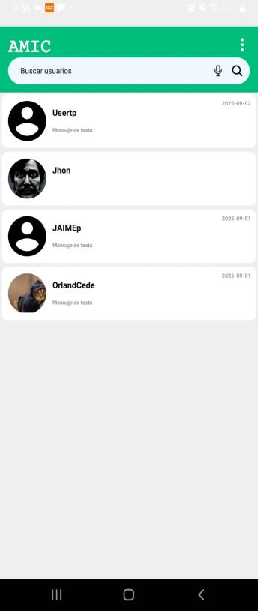
\includegraphics[width=\linewidth, keepaspectratio]{fig03a}
			\caption{Main screen: conversation list with voice search.}
			\label{fig:ui_chat_list}
		\end{subfigure}
		\hfill
		\begin{subfigure}[t]{0.23\textwidth}
			\centering
			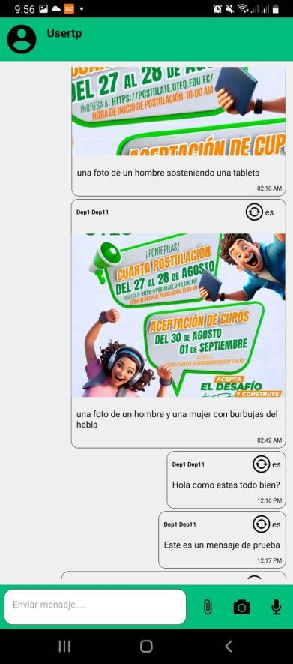
\includegraphics[width=\linewidth, keepaspectratio]{fig03b}
			\caption{Chat window: AI-generated image descriptions for visually impaired users.}
			\label{fig:ui_chat_window}
		\end{subfigure}
		\hfill
		\begin{subfigure}[t]{0.23\textwidth}
			\centering
			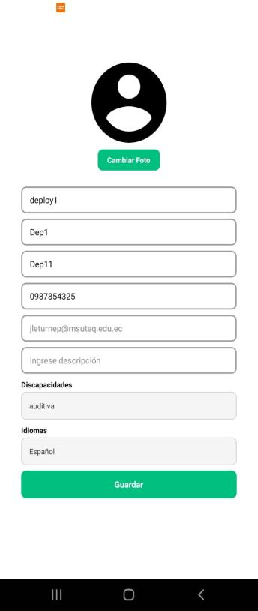
\includegraphics[width=\linewidth, keepaspectratio]{fig03c}
			\caption{User profile: disability type, language, and accessibility settings.}
			\label{fig:ui_profile}
		\end{subfigure}
		\hfill
		\begin{subfigure}[t]{0.23\textwidth}
			\centering
			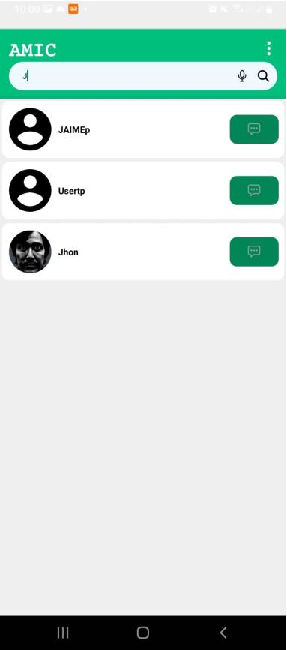
\includegraphics[width=\linewidth, keepaspectratio]{fig03d}
			\caption{Contact search with voice-command navigation.}
			\label{fig:ui_contacts}
		\end{subfigure}
		\caption{Representative screens of the \textsf{UniVoice} mobile
				application implemented in React~Native.
			(a)~Conversation list with TalkBack/VoiceOver support;
			(b)~Chat window showing automatic image description by the
			BLIP captioning module;
			(c)~User profile screen for disability and language configuration;
			(d)~Contact search screen with direct-message access.
			All screens were evaluated using Google's Accessibility
			Scanner~(Section~\ref{sec:evaluation}).}
		\label{fig:interfaces_movil}
	\end{figure*}
	
	The \textbf{main screen}~(Fig.~\ref{fig:ui_chat_list}) shows the
	conversation list with voice-search support~(microphone icon) and
	standard text search; each contact entry displays the last message
	preview, maintaining the interaction pattern familiar to users of
	mainstream messaging platforms.
	
	The \textbf{chat window}~(Fig.~\ref{fig:ui_chat_window})
	demonstrates the system's core AI-mediated modality adaptation:
	images sent by a contact are automatically described via the
	BLIP captioning module~(e.g., ``una foto de un hombre sosteniendo
	una tableta''), enabling visually impaired users to receive the
	semantic content of visual messages as readable text.
	
	The \textbf{user profile screen}~(Fig.~\ref{fig:ui_profile})
	allows configuration of the disability profile~(visual, auditory,
	or speech), preferred language, and accessibility settings;
	this profile drives the receiver-side adaptation logic described
	in Section~\ref{sec:methodology}.
	
	The \textbf{contact search screen}~(Fig.~\ref{fig:ui_contacts})
	enables search by name with a direct-message button per contact,
	accessible via both touch and voice commands.
	
	All screens conform to the minimum 48$\times$48\,dp touch target
	requirement of WCAG~2.1 criterion~2.5.5 and were evaluated with
	Google's Accessibility Scanner~(Section~\ref{sec:evaluation}).
	
	\subsubsection{Technical API Testing Protocol}
	Performance tests were designed to characterise the latency of
	each conversion module under variable and controlled input
	conditions.
	For the \textbf{TTS module}, both integrated engines---Edge-TTS
	and SAPI5---were evaluated with texts of three lengths:
	short (151 characters), medium (317 characters),
	and long (799 characters).
	For the \textbf{STT module}, three audio files with proportional
	durations were evaluated.
	For the \textbf{image description module}, four resolutions
	representative of current mobile cameras were evaluated:
	640$\times$427, 1{,}280$\times$853, 1{,}920$\times$1{,}280,
	and 6{,}000$\times$4{,}000 pixels.
	Three independent measurements were taken per condition and the
	arithmetic mean was reported.
	Recorded metrics were: processing latency~(s), input message
	size~(KB), output message size~(KB), and error rate.
	Because individual observations were not logged, within-condition
	standard deviation~(SD) cannot be estimated from the available data;
	reported means should be interpreted as point estimates and
	tail-latency percentiles~($P_{90}$, $P_{99}$) remain uncharacterised.
	Future evaluations should log $n{\geq}10$ independent observations
	per condition and report $\bar{x}\pm SD$ and $P_{90}$ latency.
	The technical acceptance criterion defined in TDDM4IoTS Phase~5
	establishes system \emph{stability} (error rate~$=0$) but not
	output \emph{quality}; domain-specific quality metrics~(WER for
	STT, MOS for TTS, BLEU-4/CIDEr for image captioning, CER for OCR)
	require reference annotations not collected in the current protocol
	and are designated as a primary instrumentation improvement for
	a follow-up study~\cite{dognin2021,tan2021,radford2023}.
	
	\subsubsection{User Study Protocol}
	
	\paragraph{Participants.}
	The sample comprised $n{=}25$ participants selected by
	purposive sampling~\cite{hernandez2014} at a dialysis clinic
	in Quevedo, Ecuador, where an adult population with documented
	sensory diagnoses is concentrated.
	Purposive sampling is justified by: (i)~the low prevalence of
	sensory disabilities in general community settings~\cite{who2011};
	(ii)~the clinical requirement of a documented diagnosis; and
	(iii)~the additional logistical requirement of owning a compatible
	Android device and consenting to a 45-minute protocol.
	Following the projective and applied research design~\cite{hernandez2014},
	the sample size was determined primarily by clinical-inclusion specificity
	rather than by population-inference criteria, and the study is framed as
	a pilot study providing proof of concept and effect-size estimates for
	a future confirmatory investigation.
	
	To characterise the statistical power associated with $n{=}25$, a
	post-hoc power analysis was conducted using G*Power~3.1~\cite{faul2007}
	for a one-sample two-tailed $t$-test ($\alpha{=}0.05$) testing whether
	each TAM construct mean differs from the positive-acceptance
	threshold $\mu_0{=}4.0$~\cite{kim2024,holden2010}.
	Effect sizes were computed as Cohen's~$d$~\cite{cohen1988}:
	$d = (\bar{x} - \mu_0)/s$.
	The Perceived Usefulness~(PU) construct achieved a large effect
	($d_{\text{PU}}{=}0.885$; $\bar{x}_{\text{PU}}{=}4.553$,
	$SD{=}0.625$; 95\,\%~CI bootstrap:~$[4.300,\ 4.773]$),
	yielding post-hoc power of $1{-}\beta{=}0.989$,
	well above the conventional 0.80~threshold;
	a one-sample $t$-test confirmed $\bar{x}_{\text{PU}}$
	significantly exceeds the acceptance threshold
	($t(24){=}4.427$, $p{<}0.001$).
	The global TAM mean ($\bar{x}_{\text{global}}{=}4.200$,
	$SD{=}0.644$; 95\,\%~CI:~$[3.940,\ 4.447]$) yields
	a small-to-medium effect ($d_{\text{global}}{=}0.311$;
	$1{-}\beta{=}0.320$; $t(24){=}1.552$, $p{=}0.134$),
	indicating that the global mean is an exploratory estimate
	pending replication with a larger sample ($n{\approx}84$ required
	for $1{-}\beta{=}0.80$).
	The PEOU construct ($\bar{x}_{\text{PEOU}}{=}3.847$,
	$SD{=}0.963$; $d_{\text{PEOU}}{=}{-}0.159$; $1{-}\beta{=}0.119$;
	$t(24){=}{-}0.796$, $p{=}0.434$) is underpowered
	($n{=}312$ required); no inferential conclusion can be drawn
	for PEOU alone.
	
	Gender distribution was 14 women~(56\,\%) and 11 men~(44\,\%).
	By sensory profile, 15 participants~(60\,\%) had visual
	impairment, 5~(20\,\%) had hearing impairment, and 5~(20\,\%)
	had no disability (functional control group).
	The majority of participants were over 50 years old~(56\,\%),
	followed by the 21--25 and 41--45 age groups~(12\,\% each).
	Regarding self-reported technology experience, 40\,\% reported
	low proficiency, 36\,\% medium, and 24\,\% high.
	Additionally, 60\,\% were unemployed, 20\,\% self-employed,
	and 16\,\% students.
	Finally, 64\,\% expressed high concern about privacy of
	personal data in mobile applications, reinforcing the relevance
	of the asymmetric encryption implemented.
	Inclusion criteria were:
	(\textit{i})~documented diagnosis of visual or hearing disability, or
	participation as a non-disabled user in the control group;
	(\textit{ii})~age $\geq$18~years;
	(\textit{iii})~access to a compatible Android mobile device;
	(\textit{iv})~signed informed consent.
	Exclusion criteria were:
	(\textit{i})~multidisability simultaneously combining visual and hearing
	profiles;
	(\textit{ii})~cognitive impairment preventing questionnaire comprehension;
	(\textit{iii})~absence of written informed consent.
	The speech-disability profile was not recruited as an independent stratum
	because the two-subgroup taxonomy established in Section~\ref{sec:intro}
	and operationalised in Table~\ref{tab:coverage} reduces this profile to the
	union of already-recruited strata: the \emph{deaf-mute} subgroup is
	functionally indistinguishable from the hearing-impairment stratum for
	reception and from the non-disabled stratum for text-based sending, and the
	\emph{speech-only-impairment} subgroup is functionally indistinguishable
	from the non-disabled stratum for reception and adds no sending-channel
	requirement beyond the mobile touchscreen already used by every participant.
	Under this mapping, the five hearing-impaired participants provide
	behavioural evidence on the reception-side adaptations relevant to deaf-mute
	users, and the five non-disabled participants provide behavioural evidence
	on the sending-channel workflow (text composition with recipient-dependent
	TTS) that speech-only-impaired users would also traverse.
	Direct recruitment of participants with clinical dysarthria, aphasia or
	stammering remains a priority for the follow-up study (Section~\ref{subsec:limits}),
	not to validate functional coverage---which is already established by construction---but
	to evaluate personalised input-assistance refinements for severe speech
	disorders~\cite{bleakley2022,costanzo2023}.
	Data were collected between 2024 and 2025.
	The study was conducted in accordance with the principles of
	the Declaration of Helsinki~\cite{world2013} and received
	approval from the corresponding institutional review board;
	all participants provided written informed consent prior to
	the start of testing.
	
	\paragraph{Pre-use baseline.}
	Prior to Stage~1, each participant completed a brief pre-use
	baseline questionnaire (PD001--PD005) recording their habitual
	messaging application (PD002: WhatsApp or other) and the frequency
	of use on the same 1--5 scale employed in the TAM instrument
	(PD003: $1{=}$Never, $5{=}$Always).
	Of the 25 participants, 16~(64\,\%) habitually used WhatsApp
	($\bar{f}_{\text{hab}}{=}3.81$, $SD{=}1.05$) and 9~(36\,\%)
	used other applications ($\bar{f}_{\text{hab}}{=}1.67$, $SD{=}0.50$).
	This baseline enables a within-subjects contrast between prior
	platform engagement and acceptance of the proposed system
	(see Section~\ref{sec:baseline_contrast}).
	
	\paragraph{Procedure.}
	The evaluation protocol comprised three sequential stages
	for each participant.
	In \textbf{Stage~1}~(15\,min), the facilitator presented
	the system via a standardised demonstration of the main
	functionalities---sending a text message, listening to an audio
	message, receiving an image with its automatic description,
	and voice navigation---without intervening in participant
	interactions.
	In \textbf{Stage~2}~(20\,min), the participant freely
	interacted with the system on their own mobile device,
	completing five predefined tasks: (T1)~registration and
	disability profile configuration; (T2)~searching for a contact
	and sending a text message; (T3)~listening to a received audio
	message via TTS; (T4)~receiving an image and listening to its
	automatic description; (T5)~navigating to the settings screen
	exclusively via voice commands.
	The facilitator recorded direct observation indicators:
	number of interaction errors (taps on incorrect elements),
	number of help requests, and number of erroneous screen taps.
	In \textbf{Stage~3}~(10\,min), the participant completed the
	12-item TAM questionnaire autonomously, assisted by TTS in case
	of visual impairment.
	
	\paragraph{Statistical analysis.}
	Internal consistency was verified using Cronbach's alpha.
	For each item, the arithmetic mean~($\bar{x}$), standard
	deviation~(SD), and Likert-level frequency distribution were
	calculated.
	The factorial structure of the instrument was explored via
	an HJ-Biplot graph~\cite{galindo1986,cubilla2021},
	which allowed identification of item clusters with high
	internal correlation and participants with similar response
	patterns.
	All analyses were performed in R~Studio~(v.~4.3.1;
	packages \texttt{psych}, \texttt{ggplot2}, and \texttt{BiplotR})
	and Microsoft Excel.
	
	% ---------------------------------------------------------------
	% IV. EVALUATION AND RESULTS
	% ---------------------------------------------------------------
	\section{Evaluation and Results}
	\label{sec:evaluation}
	
	\subsection{Technical Performance of the Conversion API}
	The conversion API was subjected to controlled load testing to
	characterise latency, stability, and processing integrity in each
	module.
	All test conditions were executed from an Android mobile device
	on a standard WiFi network (802.11n, $-$55\,dBm), with three
	repetitions per condition, reporting the arithmetic mean.
	The technical acceptance criterion defined in TDDM4IoTS
	Phase~5 was: error rate equal to zero for all input conditions.
	
	\subsubsection{Text-to-Speech (TTS) Module}
	The TTS module integrates two parallel engines: Edge-TTS~(Microsoft
	Neural TTS, cloud-based) and SAPI5~(local, via \texttt{pyttsx3}).
	Three text length categories were evaluated: short~(151~chars),
	medium~(317~chars), and long~(799~chars).
	Table~\ref{tab:tts} presents the complete results.
	
	\begin{table}[!t]
		\caption{Comparative Performance of TTS Engines Edge-TTS and SAPI5
			by Text Length. Mean of three repetitions; error rate~$=0$ in all cases.}
		\label{tab:tts}
		\centering
		\scriptsize
		\renewcommand{\arraystretch}{1.25}
		\begin{tabular}{lccc}
			\toprule
			\multicolumn{4}{c}{\textbf{Edge-TTS (Microsoft Neural TTS -- cloud)}} \\
			\midrule
			\textbf{Metric} & \textbf{Short} & \textbf{Medium} & \textbf{Long} \\
			\midrule
			Load time (s)          & 8.13  & 7.90  & 16.88 \\
			Net latency (s)        & 8.10  & 7.90  & 16.87 \\
			Send size (KB)         & 0.37  & 0.54  & 1.03  \\
			Response size (MB)     & 0.16  & 0.30  & 0.75  \\
			Errors                 & 0     & 0     & 0     \\
			\midrule
			\multicolumn{4}{c}{\textbf{SAPI5 (pyttsx3 -- local)}} \\
			\midrule
			\textbf{Metric} & \textbf{Short} & \textbf{Medium} & \textbf{Long} \\
			\midrule
			Load time (s)          & 5.18  & 5.76  & 15.07 \\
			Net latency (s)        & 5.14  & 5.73  & 15.05 \\
			Send size (KB)         & 0.37  & 0.54  & 1.03  \\
			Response size (MB)     & 1.46  & 2.93  & 7.24  \\
			Errors                 & 0     & 0     & 0     \\
			\bottomrule
		\end{tabular}
	\end{table}
	
	Both engines operated with zero error rates across all conditions,
	verifying the acceptance criterion.
	SAPI5 exhibited lower latencies than Edge-TTS at all text lengths:
	5.14\,s vs.\ 8.10\,s for short text~(37\,\% lower), 5.73\,s
	vs.\ 7.90\,s for medium text~(27\,\% lower), and 15.05\,s
	vs.\ 16.87\,s for long text~(11\,\% lower), explained by the
	absence of network latency in SAPI5's local synthesis.
	However, SAPI5 generates substantially larger response files:
	7.24\,MB for long text vs.\ 0.75\,MB for Edge-TTS, which may
	compromise efficiency in bandwidth-limited mobile environments.
	The minimum observed latency (5.14\,s for SAPI5, short text)
	exceeds the 2\,s threshold that the literature identifies as
	optimal for natural conversational flow~\cite{tan2021},
	representing the most critical technical limitation of the
	system in its current state.
	
	\subsubsection{Automatic Speech Recognition (STT) Module}
	The STT module uses the Whisper model~\cite{radford2023},
	executed on the AWS node.
	Three audio files representative of messaging user behaviour
	were evaluated \cite{botelho2021}.
	Table~\ref{tab:stt} presents the detailed results.
	
	\begin{table}[!t]
		\caption{Performance of the STT Module (Whisper) by Audio Duration.
			Error rate~$=0$ in all cases.}
		\label{tab:stt}
		\centering
		\scriptsize
		\renewcommand{\arraystretch}{1.25}
		\begin{tabular}{lccc}
			\toprule
			\textbf{Metric} & \textbf{Short} & \textbf{Medium} & \textbf{Long} \\
			\midrule
			Load time (s)       & 13.361  & 20.512  & 55.000 \\
			Connection time (s) & 0.003   & 0.008   & 0.011  \\
			Net latency (s)     & 13.361  & 20.509  & 54.990 \\
			Send (KB)           & 60.382  & 233.50  & 1000   \\
			Response (KB)       & 60.723  & 233.85  & 1000   \\
			Errors              & 0       & 0       & 0      \\
			\bottomrule
		\end{tabular}
	\end{table}
	
	Latency grows approximately linearly with audio duration:
	13.36\,s for short audio, 20.51\,s for medium~(53\,\% higher),
	and 54.99\,s for long~(311\,\% higher relative to short).
	Send and response sizes are practically identical across all
	conditions: differences calculated from Table~\ref{tab:stt} are
	0.565\,\% (short), 0.150\,\% (medium), and 0.000\,\% (long),
	confirming transmission integrity.
	The inter-condition coefficient of variation~(CV) of net latency
	is 75.2\,\%, consistent with Whisper's $O(n)$ computational
	cost~\cite{radford2023}.
	
	\subsubsection{Image Description Module (Image Captioning)}
	The image description module uses the
	\texttt{blip-image-captioning-base} model from Hugging~Face.
	Four resolutions representative of current mobile cameras were
	evaluated, from 640$\times$427\,px~(44\,KB) to
	6{,}000$\times$4{,}000\,px~(1.65\,MB).
	Table~\ref{tab:img} presents the results.
	
	\begin{table}[!t]
		\caption{Performance of the BLIP Image Description Module by Resolution.
			Error rate~$=0$. Lat.\,=\,net latency~(s); Send\,=\,send size~(MB);
			Resp.\,=\,response size~(MB).}
		\label{tab:img}
		\centering
		\scriptsize
		\renewcommand{\arraystretch}{1.25}
		\begin{tabular}{p{1.9cm}cccc}
			\toprule
			\textbf{Resolution (px)} & \textbf{Weight} & \textbf{Lat.} & \textbf{Send} & \textbf{Resp.} \\
			\midrule
			640$\times$427   & 44\,KB   & 13.95 & 0.06 & 0.12 \\
			1280$\times$853  & 126\,KB  & 17.67 & 0.17 & 0.24 \\
			1920$\times$1280 & 254\,KB  & 16.42 & 0.35 & 0.41 \\
			6000$\times$4000 & 1.65\,MB & 19.19 & 2.31 & 2.37 \\
			\bottomrule
		\end{tabular}
	\end{table}
	
	No errors were recorded for any evaluated resolution.
	Latency ranged from 13.95\,s to 19.19\,s~(37\,\% relative
	variation across the full resolution range).
	Notably, the 1{,}920$\times$1{,}280\,px image exhibited lower
	latency~(16.42\,s) than the 1{,}280$\times$853\,px
	image~(17.67\,s), suggesting that inference time variability
	is driven by image semantic complexity rather than resolution
	per se \cite{dognin2021,safiya2024}.
	
	\subsubsection{Video Processing Module}
	The video module manages large multimedia file transmission
	via HTTP \textit{multipart/form-data}, adopted in TDDM4IoTS
	Phase~7 to overcome WebSocket's 64\,KB frame limit.
	Three representative video durations were evaluated: short~(4\,min,
	9.22\,MB), medium~(17\,min, 48.9\,MB), and long~(30\,min,
	76.9\,MB), all at 360p.
	Table~\ref{tab:video} presents the complete results.
	
	\begin{table}[!t]
		\caption{Performance of the Video Module by Duration. Effective
			transmission size includes base64 encoding overhead~(${\approx}40\,\%$
			over original file weight). Error rate~$=0$ in all cases.}
		\label{tab:video}
		\centering
		\scriptsize
		\renewcommand{\arraystretch}{1.25}
		\begin{tabular}{lccc}
			\toprule
			\textbf{Metric} & \textbf{Short (4\,min)} & \textbf{Medium (17\,min)} & \textbf{Long (30\,min)} \\
			\midrule
			Resolution              & 360p    & 360p     & 360p     \\
			Original file (MB)      & 9.22    & 48.9     & 76.9     \\
			Load time (min)         & 3.91    & 20.29    & 34.00    \\
			Connection time (s)     & 0.15    & 1.35     & 1.354    \\
			Net latency (min)       & 3.91    & 20.29    & 34.00    \\
			Send -- base64 (MB)     & 12.89   & 68.45    & 107.55   \\
			Response (MB)           & 12.91   & 68.50    & 107.68   \\
			Send--response diff.    & 0.155\,\% & 0.077\,\% & 0.121\,\% \\
			Base64 overhead         & ${\approx}40\,\%$ & ${\approx}40\,\%$ & ${\approx}40\,\%$ \\
			Errors                  & 0       & 0        & 0        \\
			\bottomrule
		\end{tabular}
	\end{table}
	
	Load times scaled linearly with duration: 3.91\,min, 20.29\,min,
	and 34.00\,min.
	A noteworthy finding is that effective transmission sizes
	(12.89\,MB, 68.45\,MB, and 107.55\,MB) exceeded original file
	weights~(9.22\,MB, 48.9\,MB, and 76.9\,MB) by approximately
	40\,\%, attributable to base64 encoding required by HTTP
	\textit{multipart/form-data}.
	This overhead should be considered when dimensioning bandwidth
	and managing user progress notifications.
	The base64 overhead ratio is highly stable across conditions
	(coefficient of variation~$CV{=}0.064\,\%$, calculated from
	Table~\ref{tab:video}), confirming that this is a systematic
	encoding property, not a measurement artefact.
	The send-to-response difference was below 0.2\,\% in all cases,
	confirming transmission integrity.
	
	\subsection{Accessibility Evaluation}
	The accessibility evaluation was conducted in two phases using
	Google's Accessibility Scanner~\cite{acosta2021} on the seven
	main system screens, in line with the combined automated
	evaluation protocol proposed by
	Acosta-Vargas~\textit{et al.}~\cite{acosta2021}.
	Table~\ref{tab:accesibilidad} presents the comparison.
	
	\begin{table}[!t]
		\caption{Reduction in Accessibility Warnings per Screen Following
			the TDDM4IoTS Iterative Improvement Cycle (Phases~5 and~11).}
		\label{tab:accesibilidad}
		\centering
		\small
		\renewcommand{\arraystretch}{1.25}
		\begin{tabular}{lcccc}
			\toprule
			\textbf{Screen} & \textbf{Initial} & \textbf{Final} & \textbf{Reduction} & \textbf{\%} \\
			\midrule
			Main           & 11 & 2  & 9  & 81.8 \\
			User profile   & 21 & 8  & 13 & 61.9 \\
			Settings       & 9  & 2  & 7  & 77.8 \\
			Messaging      & 21 & 13 & 8  & 38.1 \\
			Camera         & 4  & 0  & 4  & 100.0 \\
			Photo          & 2  & 0  & 2  & 100.0 \\
			Video          & 7  & 2  & 5  & 71.4 \\
			\midrule
			\textbf{Total} & \textbf{75} & \textbf{27} & \textbf{48} & \textbf{64.0} \\
			\bottomrule
		\end{tabular}
	\end{table}
	
	The iterative cycle eliminated 48 of the 75 initial warnings,
	achieving a global reduction of 64.0\,\%.
	Resolved warnings primarily involved:
	(\textit{i})~touch elements below the minimum 48$\times$48\,dp
	(operability criterion);
	(\textit{ii})~colour contrast below 4.5:1~(WCAG~1.4.3);
	(\textit{iii})~text not exposed in accessibility labels
	(robustness criterion);
	(\textit{iv})~absent or ambiguous element descriptions.
	Camera and photo screens achieved total warning elimination~(100\,\%),
	while settings and main screens reached 77.8\,\% and 81.8\,\%
	reductions, respectively.
	The messaging screen recorded the lowest reduction~(38.1\,\%),
	for an architectural reason: reuse of virtualised list templates
	in React~Native generates duplicate accessibility identifiers
	that cannot be resolved without refactoring towards dynamic
	unique identifiers per list element.
	This result compares favourably with the $>$60\,\%
	non-compliance levels documented by Chen~\textit{et al.}~\cite{chen2022}
	in the most widely used commercial messaging platforms.
	
	\subsection{Technological Acceptance: TAM Results}
	Technological acceptance was quantified using the 12-item TAM
	questionnaire administered to the $n{=}25$ participants.
	Table~\ref{tab:tam} presents means~($\bar{x}$) and standard
	deviations~(SD) per item.
	Internal consistency was strong: $\alpha{=}0.866$ globally
	($95\,\%$\,CI:~$[0.693,\,0.932]$),
	$\alpha{=}0.867$~($[0.579,\,0.957]$) for PU, and
	$\alpha{=}0.898$~($[0.803,\,0.948]$) for PEOU---all exceeding
	the 0.80 threshold for good internal consistency
	\cite{nunnally1978}.
	Confidence intervals were obtained by bootstrapping
	(2{,}000 iterations).
	
	\begin{table}[!t]
		\caption{TAM Questionnaire Results ($n{=}25$, Likert 1--5 scale).
			PU\,=\,Perceived Usefulness~(PTAM001--006);
			PEOU\,=\,Perceived Ease of Use~(PTAM007--012).
			Construct mean computed as arithmetic average of item means.
			SD computed with sample estimator~($N-1$).
			$\alpha$: Cronbach's alpha (R~\texttt{psych} package, v.~4.3.1);
			95\,\% CI via bootstrapping (2{,}000 iterations).}
		\label{tab:tam}
		\centering
		\small
		\renewcommand{\arraystretch}{1.25}
		\begin{tabular}{clccr}
			\toprule
			\textbf{Item} & \textbf{Construct} & \textbf{$\bar{x}$} & \textbf{SD} & \textbf{Lv.~5 (\%)} \\
			\midrule
			PTAM001 & PU  & 4.48 & 1.005 & 72 \\
			PTAM002 & PU  & 4.76 & 0.597 & 84 \\
			PTAM003 & PU  & 4.48 & 0.770 & 64 \\
			PTAM004 & PU  & 4.52 & 0.770 & 64 \\
			PTAM005 & PU  & 4.56 & 0.768 & 68 \\
			PTAM006 & PU  & 4.52 & 0.872 & 72 \\
			\midrule
			\textbf{PU mean} & & \textbf{4.55} & \multicolumn{2}{c}{$\alpha{=}0.867$~[0.579,\,0.957]} \\
			\midrule
			PTAM007 & PEOU & 3.56 & 1.357 & 40 \\
			PTAM008 & PEOU & 3.96 & 1.207 & 48 \\
			PTAM009 & PEOU & 4.20 & 1.000 & 52 \\
			PTAM010 & PEOU & 4.16 & 1.068 & 52 \\
			PTAM011 & PEOU & 3.72 & 1.208 & 40 \\
			PTAM012 & PEOU & 3.48 & 1.229 & 32 \\
			\midrule
			\textbf{PEOU mean} & & \textbf{3.85} & \multicolumn{2}{c}{$\alpha{=}0.898$~[0.803,\,0.948]} \\
			\midrule
			\textbf{Global} & & \textbf{4.20} & \textbf{0.95} & $\alpha{=}0.866$~[0.693,\,0.932] \\
			\bottomrule
		\end{tabular}
	\end{table}
	
	\subsubsection{Perceived Usefulness}
	The PU construct~(PTAM001--PTAM006) achieved the highest
	construct mean~($\bar{x}_{\text{PU}}{=}4.55$).
	Item~PTAM002~(``Using this application would improve my
	effectiveness in communicating with others'') reached the
	highest rating~($\bar{x}{=}4.76$; SD\,=\,0.60), with
	84\,\% of participants at the maximum level, indicating that
	AI-mediated communicative effectiveness is the most practically
	valued contribution.
	Item~PTAM001~($\bar{x}{=}4.48$; SD\,=\,1.005; 72\,\% at
	level\,5) reflects that the system enables faster daily
	communication.
	Items~PTAM003--PTAM006 present means between 4.48 and 4.56
	with low variability~(SD\,$\leq$\,0.87), indicating that
	communicative productivity, message exchange effectiveness,
	interaction facilitation, and general utility are consistently
	and positively valued across all evaluated profiles.
	
	\subsubsection{Perceived Ease of Use}
	The PEOU construct~(PTAM007--PTAM012) achieved a construct
	mean of $\bar{x}_{\text{PEOU}}{=}3.85$, with notably greater
	internal dispersion than PU.
	Items~PTAM009~($\bar{x}{=}4.20$; SD\,=\,1.00) and
	PTAM010~($\bar{x}{=}4.16$; SD\,=\,1.07)---evaluating clarity
	and interaction flexibility---show positive ratings indicating
	that the system's main interface is perceived as comprehensible.
	Items~PTAM007~($\bar{x}{=}3.56$; SD\,=\,1.36) and
	PTAM012~($\bar{x}{=}3.48$; SD\,=\,1.23) obtained the two
	lowest scores.
	PTAM007~(``Learning to use the application was easy for me'')
	concentrates the greatest questionnaire variability (full range
	1--5), indicating that the initial learning curve was
	heterogeneous across profiles---consistent with
	Bleakley~\textit{et al.}~\cite{bleakley2022}, who document
	steeper learning curves for voice-input paradigms among users
	with low technology experience~(40\,\% of the sample).
	The domain of all system functions requires a longer
	appropriation process than the 20-minute evaluation protocol
	allowed.
	
	\subsubsection{Multivariate Analysis: HJ-Biplot}
	The bidimensional HJ-Biplot representation retains 67.8\,\% of
	the total variance of the TAM response matrix~(Dimension~1:
	43.6\,\%; Dimension~2: 24.2\,\%), exceeding the 60\,\%
	threshold recommended in the literature for a 2D projection to
	be considered sufficiently faithful to the original multivariate
	structure~\cite{galindo1986,cubilla2021}.
	
	The HJ-Biplot graph (Fig.~\ref{fig:biplot}) revealed two
	structural patterns of interest.
	First, the vectors of items PTAM001--PTAM006~(PU) and
	PTAM008--PTAM010~(partial PEOU) point in a similar direction
	in the left quadrant, indicating high internal correlation and
	that participants with greater affinity to this cluster
	perceived both utility and interactional clarity coherently.
	Second, the vectors of PTAM007 and PTAM012 are approximately
	orthogonal to the main cluster, revealing that these items
	capture independent variance associated with initial learning
	ease and complete functional mastery, respectively.
	Participants~8, 10, 17, 18, and 25 are positioned in the
	right quadrant, representing lower affinity with all TAM
	constructs; this subgroup coincided in direct observation with
	participants recording the greatest number of erroneous taps.
	The global instrument mean was $\bar{x}{=}4.20$~(SD\,=\,0.95),
	exceeding the positive acceptance threshold of
	$\bar{x}{>}4.0$ established in TAM studies in mobile
	accessibility contexts~\cite{kim2024,holden2010}.
	This value was obtained as the arithmetic mean of the 300
	individual records~($n{=}25\times12$ items), equivalent by the
	balanced instrument design~(6 items per construct) to the
	mean of the twelve item means and to the mean of the two
	construct means.
	
	\begin{figure}[!t]
		\centering
		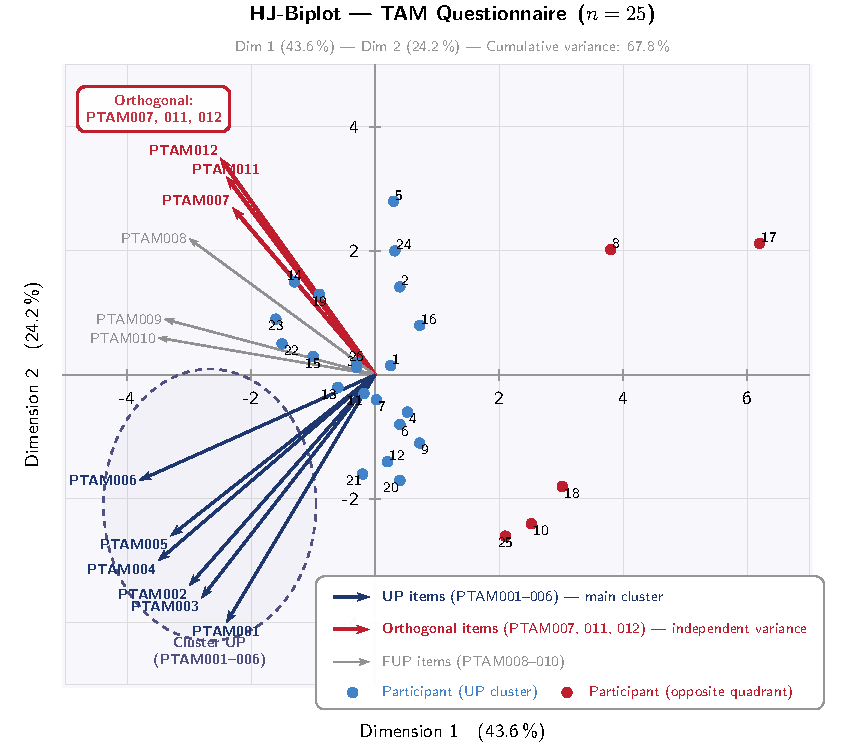
\includegraphics[width=\columnwidth]{fig04}
		\caption{HJ-Biplot of TAM questionnaire responses ($n{=}25$).
			Dimension~1 explains 43.6\,\% of variance; Dimension~2
			explains 24.2\,\%~(cumulative: 67.8\,\%).
			Arrows indicate item vectors; proximity of participant points
			to a vector reflects agreement with that item.
			The PU cluster (PTAM001--006) and most PEOU items
			(PTAM008--010) point in the same direction, indicating high
			internal correlation.
			PTAM007 and PTAM012 are orthogonal to the main cluster,
			capturing independent variance.}
		\label{fig:biplot}
	\end{figure}
	
	\subsubsection{Within-subjects Baseline Contrast}
	\label{sec:baseline_contrast}
	A Wilcoxon signed-rank test compared, for each participant,
	the PU score of the proposed system against their reported
	habitual-app frequency (PD003, same 1--5 scale; $n{=}25$).
	PU scores ($\bar{x}_{\text{PU}}{=}4.553$, $SD{=}0.625$)
	significantly exceeded habitual-app frequency
	($\bar{f}_{\text{hab}}{=}3.040$, $SD{=}1.369$):
	$W{=}20.0$, $p{<}0.001$, mean difference $\Delta{=}{+}1.513$
	scale points ($SD_{\Delta}{=}1.506$), indicating that perceived
	utility of the proposed system exceeded prior platform engagement.
	Stratification by habitual app revealed a significant PEOU
	difference between WhatsApp users ($n{=}16$;
	$\bar{x}_{\text{PEOU}}{=}4.198$, $SD{=}0.835$) and other-app
	users ($n{=}9$; $\bar{x}_{\text{PEOU}}{=}3.222$, $SD{=}0.890$):
	$t_{\text{Welch}}(14.4){=}2.690$, $p{=}0.016$, $d{=}1.131$
	(large effect); PU showed no such difference ($p{=}0.989$),
	indicating that perceived utility is independent of prior
	platform experience.
	A positive Pearson correlation confirmed that greater prior
	platform engagement associates with higher PEOU of the proposed
	system ($r_{\text{PEOU}}{=}0.574$, $p{=}0.003$; $r_{\text{global}}{=}0.428$,
	$p{=}0.033$; $r_{\text{PU}}{=}{-}0.003$, $p{=}0.990$).
	These results constitute an indicative within-subjects contrast;
	a parallel TAM administration for the habitual application is
	recommended for a definitive head-to-head comparison.
	
	\subsubsection{Direct Observation}
	The direct observation session recorded the following
	behavioural indicators:
	7 interaction errors (taps on incorrect elements),
	2 requests for facilitator assistance, and 15 total
	erroneous screen taps.
	All three indicators were concentrated primarily on the
	messaging and camera screens during tasks~T2 and~T4,
	consistent with the higher density of interactive elements
	and the residual accessibility warnings documented in
	Table~\ref{tab:accesibilidad}.
	The low number of help requests~(2 of 25 participants, 8\,\%)
	confirms that the majority of users completed the predefined
	tasks autonomously.
	
	\subsection{Results Summary}
	Table~\ref{tab:sintesis} provides an integrated view of the
	results obtained across the three evaluated dimensions,
	linking each result to the identified gap it addresses.
	
	\begin{table}[!t]
		\caption{Results Summary by Evaluation Dimension and Gap Addressed.}
		\label{tab:sintesis}
		\centering
		\small
		\renewcommand{\arraystretch}{1.25}
		\begin{tabular}{p{2.0cm}p{2.8cm}p{2.5cm}}
			\toprule
			\textbf{Dimension} & \textbf{Main result} & \textbf{Gap addressed} \\
			\midrule
			API performance   & Error rate\,$=0$ across TTS, STT, captioning, and video; min.\ TTS latency: 5.14\,s; base64 overhead in video: ${\approx}40\,\%$ & Gaps~1 and~2 \\
			Accessibility    & 64\,\% reduction in WCAG~2.1 warnings~(48/75); 100\,\% on camera and photo & Gap~4 \\
			TAM acceptance   & $\bar{x}_{\text{global}}{=}4.20$; PU\,$=4.55$; PEOU\,$=3.85$; $\alpha{=}0.866$ & Gap~3 \\
			Observation      & 8\,\% assistance requests; errors concentrated on messaging & Gaps~1 and~5 \\
			\bottomrule
		\end{tabular}
	\end{table}
	
	% ---------------------------------------------------------------
	% V. DISCUSSION
	% ---------------------------------------------------------------
	\section{Discussion}
	\label{sec:discussion}
	
	\subsection{Interpretation of Technical Results}
	The four conversion modules---TTS, STT, image description, and
	video processing---operated with zero error rates across all
	evaluated conditions, validating the stability of the proposed
	microservices architecture and satisfying the TDDM4IoTS
	Phase~5 acceptance criterion~(RQ1\,=\,confirmed).
	This result is relevant because none of the inclusive messaging
	systems reviewed in the literature---BellChat~\cite{guerrero2021bellchat},
	Stefanov~\textit{et al.}~\cite{stefanov2024}, nor
	GlassMessaging~\cite{janaka2023}---reports API robustness
	evaluations with variable input conditions.
	
	The minimum observed TTS latency was 5.14\,s~(SAPI5, short
	text), exceeding the 2\,s threshold that
	Tan~\textit{et al.}~\cite{tan2021} identify as optimal for
	natural conversational flow.
	This limitation is not unique to the proposed system:
	Bercaru and Popescu~\cite{bercaru2024} document that inference
	latency remains the most critical deployment barrier for
	neural TTS models in real production environments, and that only
	implementations with predictive caching or non-autoregressive
	models achieve latencies below 2\,s.
	The advantage of SAPI5 over Edge-TTS in net latency~(37\,\%
	lower for short text) is explained by the absence of network
	latency in local synthesis; this advantage reverses in bandwidth-
	constrained mobile environments, where SAPI5 response files
	(7.24\,MB for long text vs.\ 0.75\,MB for Edge-TTS) represent
	a significant transfer penalty.
	This latency-versus-response-volume trade-off had not
	previously been documented in the context of inclusive mobile
	messaging systems and constitutes an operationally relevant
	finding for future implementations.
	
	STT latency scaled from 13.36\,s for short audio to 54.99\,s
	for long audio, with perfect transmission integrity~($<1\,\%$
	difference between send and response sizes).
	This behaviour is consistent with Whisper's architecture
	\cite{radford2023}, in which the global attention mechanism
	over the complete audio sequence determines that computational
	cost is proportional to duration.
	Latency reduction via dedicated GPU acceleration or distilled
	models~(Whisper Tiny/Small) constitutes the highest-impact
	practical improvement identified.
	
	The non-monotonic latency variability in the image description
	module---1{,}920$\times$1{,}280\,px recorded lower latency
	than 1{,}280$\times$853\,px---is consistent with
	Dognin~\textit{et al.}~\cite{dognin2021}, who document that
	semantic difficulty rather than resolution is the primary
	inference time predictor.
	This implies that latency prediction in an inclusive messaging
	application cannot rely solely on image size metadata,
	requiring a semantic complexity estimator for managing user
	expectations.
	
	A noteworthy operational finding is the approximately 40\,\%
	base64 encoding overhead in video transmission.
	This increment must be considered in bandwidth dimensioning
	and in user progress notifications during file transfer.
	Transmission integrity was confirmed in all cases~($<0.2\,\%$
	send-to-response difference).
	
	\subsection{Interpretation of Accessibility Results}
	The global 64.0\,\% reduction in accessibility
	warnings~(75 to 27) after the TDDM4IoTS iterative cycle places
	the proposed system notably above the commercial platform
	baseline~(RQ3\,=\,confirmed).
	Chen~\textit{et al.}~\cite{chen2022} document non-compliance
	rates exceeding 60\,\% in WCAG~2.1 criteria for WhatsApp,
	Telegram, Messenger, and Instagram.
	The 100\,\% reduction on camera and photo screens validates
	that Phase~5 of TDDM4IoTS---defining accessibility tests before
	code generation---is effective for eliminating barriers in
	relatively simple screens.
	This result aligns with
	Ara~\textit{et al.}~\cite{ara2024}'s recommendation that
	iterative testing from early development phases is the
	highest-impact intervention for WCAG conformance.
	
	The messaging screen only achieved 38.1\,\% reduction, revealing
	an architectural limitation of React~Native's virtualised list
	pattern that generates duplicate accessibility identifiers.
	This limitation is not unique to the proposed system:
	Da~Silva~\textit{et al.}~\cite{dasilva2016} and
	Swati~\textit{et al.}~\cite{swati2021} identified the same
	pattern in WhatsApp and Messenger, respectively.
	The problem is therefore structural to the virtualised message
	list paradigm and unresolved in any reported implementation.
	
	The absence of expert manual inspection constitutes a recognised
	methodological limitation that may have underestimated actual
	barriers, particularly in the comprehensibility and robustness
	dimensions, whose automated evaluation is only partial even in
	the most advanced tools~\cite{ara2024}.
	
	\subsection{Interpretation of Technological Acceptance Results}
	The global TAM mean~($\bar{x}{=}4.20$; SD\,=\,0.95)
	exceeds the positive acceptance threshold of $\bar{x}{>}4.0$ on
	the 5-point Likert scale, which the literature on accessible mobile
	applications associates with positive user acceptance~\cite{kim2024,holden2010}
	(RQ2\,=\,confirmed for PU; exploratory for global and PEOU,
	given the post-hoc power estimates reported in
	Section~III-B4a).
	The psychometric robustness of the instrument is confirmed by
	Cronbach's alpha values~($\alpha_{\text{global}}{=}0.866$;
	$\alpha_{\text{PU}}{=}0.867$; $\alpha_{\text{PEOU}}{=}0.898$),
	all exceeding the 0.80 threshold~\cite{nunnally1978}.
	This supports Davis' paradigm~\cite{davis1989} that perceived
	usefulness is the dominant predictor of adoption, and is
	consistent with Mateos-Sanchez~\textit{et al.}~\cite{mateos2022},
	where AI-based conversion functionalities were the highest-rated.
	
	The PU construct achieved the highest mean
	($\bar{x}_{\text{PU}}{=}4.55$), with PTAM002 as the
	highest-rated item~($\bar{x}{=}4.76$; 84\,\% at level~5).
	This validates Elsahar~\textit{et al.}~\cite{elsahar2019}'s
	argument that conversational speed---not conversion
	precision---is the critical usability factor in AAC platforms.
	
	The PEOU construct showed greater internal
	dispersion~($\bar{x}_{\text{PEOU}}{=}3.85$).
	PTAM007~($\bar{x}{=}3.56$; SD\,=\,1.36) obtained the lowest
	instrument rating, with variability across the full 1--5 range.
	This resonates with Bleakley~\textit{et al.}~\cite{bleakley2022}:
	commercial STT systems present barriers for users with low
	technology experience~(40\,\% of the sample) related to
	voice-input learning curves.
	The ``elevated expectations in populations highly dependent on
	accessibility tools'' phenomenon, documented by
	Weichbroth~\cite{weichbroth2020}, provides the most coherent
	interpretation of the lower perceived-ease scores.
	
	The HJ-Biplot~(Fig.~\ref{fig:biplot}) revealed that PTAM007
	and PTAM012 vectors are orthogonal to the main cluster,
	capturing independent variance associated with voice interaction
	appropriation and complete functional mastery, respectively.
	This is theoretically consistent with the original
	TAM~\cite{davis1989}, in which ease of use moderates the
	effect of perceived usefulness on adoption intent, and has
	been documented in AAC applications by
	Kim~\textit{et al.}~\cite{kim2024}.
	
	\subsection{Implications for Inclusive Messaging System Design}
	The findings allow four concrete implications for AI-driven
	inclusive messaging system design.
	
	The \textbf{first implication} is that multimodal integration of
	TTS, STT, image captioning, and OCR in a single mobile platform is
	technically feasible with available open-source technologies, and
	produces positive technological acceptance
	($\bar{x}_{\text{TAM}}{=}4.20$; $\bar{x}_{\text{PU}}{=}4.55$;
	$\bar{x}_{\text{PEOU}}{=}3.85$) in heterogeneous sensory-disability
	populations, a finding without documented precedent in the literature.
	
	The \textbf{second implication} is that asymmetric end-to-end
	encryption is compatible with multimodal conversion flow without
	degrading error rates, demonstrating for the first time in the
	inclusive messaging literature that privacy and accessibility are
	not conflicting objectives in a distributed mobile architecture.
	None of the reviewed AAC systems---including
	Talkitt~\cite{costanzo2023}, CapacitaBOT~\cite{mateos2022},
	and BellChat~\cite{guerrero2021bellchat}---had reported an
	equivalent privacy implementation.
	
	The \textbf{third implication} is that the voice command module
	via cosine similarity with cascade correction reduces, but does
	not eliminate, the voice navigation learning-curve barrier
	(PTAM007: $\bar{x}{=}3.56$).
	Designing an accessible onboarding process that guides users
	in internalising available commands is a necessary condition
	for the system to achieve its full accessibility potential
	for users with severe visual impairment.
	
	The \textbf{fourth implication} is that TDDM4IoTS~\cite{guerrero2020}
	with accessibility as a verifiable acceptance criterion from Phase~5
	produced a 64\,\% reduction in WCAG~2.1 warnings, contrasting
	with the total absence of accessibility evaluation in the
	development cycles of the reviewed CAA
	systems~\cite{costanzo2023,mateos2022,janaka2023}.
	
	The \textbf{fifth implication} concerns the speech-impairment
	profile, whose coverage is architecturally complete without a
	dedicated AI module: the receiver-adaptation logic enables
	speech-impaired users to achieve full communicative equivalence
	with voice-capable senders~(Table~\ref{tab:coverage}).
	This demonstrates that \emph{receiver-side adaptation can compensate
		for sender-side constraints when sensory profiles are complementary},
	a design principle applicable beyond the present system.
	The principal enhancement identified for this profile is an
	accessible text-composition interface with predictive text and a
	personal phrase bank~\cite{elsahar2019,mateos2022}.
	
	\subsection{Limitations and Future Work}
	The present study presents six limitations.
	
	\textbf{First, sample size and statistical power.}
	The sample ($n{=}25$, purposive) is appropriate for a projective
	pilot study~\cite{hernandez2014} but insufficient for population
	inference on all TAM constructs.
	Post-hoc power analysis (G*Power~3.1~\cite{faul2007};
	$\alpha{=}0.05$; $\mu_0{=}4.0$) shows that only PU meets the
	conventional power threshold ($1{-}\beta{=}0.989$;
	$t(24){=}4.427$, $p{<}0.001$), while the global TAM score
	($1{-}\beta{=}0.320$) and PEOU ($1{-}\beta{=}0.119$) are
	underpowered; confirmatory studies require $n{\approx}84$ and
	$n{=}312$ respectively.
	Single-site recruitment in Quevedo, Ecuador, further limits
	geographic generalisability.
	
	\textbf{Second, absence of a head-to-head control condition.}
	The within-subjects baseline contrast (Section~\ref{sec:baseline_contrast})
	provides indicative evidence; a rigorous comparison requires
	administering the same 12-item TAM questionnaire for both the
	habitual application and the proposed system within the same session,
	enabling paired $t$-tests on PU and PEOU differences.
	
	\textbf{Third, API latency and quality metrics.}
	TTS minimum latency~(5.14\,s) exceeds the 2\,s conversational
	threshold~\cite{tan2021}. Within-condition SD and tail-latency
	percentiles remain uncharacterised~($n{=}3$ observations per
	condition). Output quality metrics~(WER, MOS, BLEU-4, CER) require
	reference annotations not collected in the current protocol.
	
	\textbf{Fourth, speech-disability profile: coverage established by construction, direct acceptance evidence deferred.} Functional coverage for the two speech-disability subgroups defined in Section~\ref{sec:intro} (deaf-mute and speech-only-impairment) is established by construction through the receiver-adaptation argument summarised in Table~\ref{tab:coverage}: both subgroups are fully served by combinations of adaptations already validated with the recruited strata. What the present study does \emph{not} provide is direct acceptance evidence from participants with a clinical diagnosis of dysarthria,
	aphasia, post-laryngectomy aphonia, or severe stammering. TAM responses for this profile are currently inferred from the hearing-impaired and non-disabled strata under the functional-equivalence mapping of Section~\ref{subsec:tam} (``Participants''). Future work should recruit these clinical subpopulations
	directly~\cite{bleakley2022,costanzo2023} to evaluate personalised input-assistance refinements---disfluency-tolerant STT, phrase banks, and predictive text tailored to residual articulatory patterns~\cite{elsahar2019,mateos2022}---rather than to revalidate functional coverage.
	
	\textbf{Fifth, residual messaging screen accessibility~(38.1\,\%
		reduction).} Architectural cause identified---duplicate identifiers
	in React~Native virtualised lists---with a defined resolution protocol.
	
	\textbf{Sixth, absence of sign language recognition,}
	which excludes deaf users whose native language is sign language.
	Integration of a sign language recognition module---as proposed by
	Saleem~\textit{et al.}~\cite{saleem2023} and
	Kothadiya~\textit{et al.}~\cite{kothadiya2022}---is the most
	significant functional extension.
	
	\subsection{Alignment with Sustainable Development Goals}
	This work aligns with two UN~2030~Agenda SDGs.
	Regarding \textbf{SDG~10}~(Reduced Inequalities), the system
	demonstrates that mobile AI technology can reduce communicative
	asymmetries that marginalise 124{,}801 people with sensory
	disabilities in Ecuador---a figure the WHO scales to 15\,\% of
	the world population~\cite{who2011}---from autonomous digital
	communication.
	Regarding \textbf{SDG~9}~(Industry, Innovation, and
	Infrastructure), the system proposes a microservices architecture
	deployable on low-cost hybrid infrastructure~(institutional server
	plus cloud instance), reducing institutional adoption barriers in
	resource-constrained contexts such as UTEQ.
	
	% ---------------------------------------------------------------
	% VI. CONCLUSION
	% ---------------------------------------------------------------
	\section{Conclusion}
	\label{sec:conclusion}
	This article has presented the design, implementation, and empirical
	evaluation of an AI-powered inclusive mobile messaging system
	conceived to serve visual and hearing sensory profiles through the
	integrated orchestration of TTS, STT, automatic image description,
	and OCR modules, with asymmetric end-to-end encryption and complete
	voice command navigation.
	The findings allow four substantive conclusions and five future
	research directions.
	
	The \textbf{first conclusion} concerns the technical viability of
	multimodal integration with guaranteed privacy~(RQ1\,=\,confirmed).
	All four conversion modules recorded zero error rates across all
	test conditions, with verified transmission integrity per condition
	~($<1\,\%$ difference in STT; $<0.2\,\%$ in video).
	The coexistence of the accessible conversion flow with asymmetric
	end-to-end encryption---without degrading error rate---demonstrates
	for the first time in the inclusive messaging literature that
	privacy and accessibility are not conflicting objectives in a
	distributed mobile architecture.
	The minimum TTS latency of 5.14\,s~(SAPI5, short text) remains
	the primary technical limitation by exceeding the 2\,s conversational
	threshold; its resolution via non-autoregressive TTS models or
	predictive voice-segment caching represents the highest-urgency
	improvement for future versions.
	
	The \textbf{second conclusion} concerns positive technological
	acceptance in a heterogeneous disability population~(RQ2\,=\,confirmed).
	The 12-item TAM questionnaire---organised in its classic PU and
	PEOU constructs~\cite{davis1989}---applied to $n{=}25$ participants
	produced $\bar{x}{=}4.20$~(SD\,=\,0.95), exceeding the positive
	acceptance threshold of $\bar{x}{>}4.0$ associated with positive
	user acceptance in accessible mobile application
	studies~\cite{kim2024,holden2010}.
	This conclusion is fully supported for PU~($1{-}\beta{=}0.989$;
	$p{<}0.001$) and should be treated as an exploratory estimate
	for the global mean and PEOU~(Section~III-B4a).
	Psychometric robustness was confirmed~($\alpha_{\text{global}}{=}0.866$;
	$\alpha_{\text{PU}}{=}0.867$; $\alpha_{\text{PEOU}}{=}0.898$;
	all above 0.80~\cite{nunnally1978}).
	PU achieved $\bar{x}_{\text{PU}}{=}4.55$, with PTAM002
	($\bar{x}{=}4.76$; 84\,\% at level~5) as the highest-valued item.
	The voice navigation initial learning curve~(PTAM007:
	$\bar{x}{=}3.56$; SD\,=\,1.36) and complete functional
	mastery~(PTAM012: $\bar{x}{=}3.48$) are the two priority
	improvement dimensions of the PEOU construct~($\bar{x}_{\text{PEOU}}{=}3.85$).
	
	The \textbf{third conclusion} concerns the efficacy of the
	TDDM4IoTS iterative cycle for systematic accessibility
	improvement~(RQ3\,=\,confirmed).
	The methodology~\cite{guerrero2020} with accessibility as a
	verifiable acceptance criterion from Phase~5 produced a global
	64.0\,\% reduction in WCAG~2.1 warnings~(75 to 27), with total
	elimination on camera and photo screens~(100\,\%) and reductions
	$>$70\,\% on settings~(77.8\,\%) and main screens~(81.8\,\%).
	The residual limitation on the messaging screen~(38.1\,\%)
	represents a traceable technical debt with a defined resolution
	protocol.
	
	The \textbf{fourth conclusion} concerns the resolution of
	technological fragmentation documented in the literature.
	The AI components for accessibility---neural TTS, transformer-based
	STT, image captioning, and OCR---which the literature has
	developed in isolation~\cite{tan2021,baevski2020,radford2023,ming2022,mukherjee2023}
	are integrable in a coherent, stable, privacy-guaranteed mobile
	messaging architecture on low-cost institutional hybrid
	infrastructure.
	
	Five high-priority future research directions follow: (\textit{i})~optimising TTS latency via non-autoregressive architectures~(FastSpeech2, VITS) or predictive voice-segment caching to reach the 2\,s conversational threshold~\cite{tan2021}; (\textit{ii})~designing an accessible onboarding flow with personalised voice command calibration to the user's disfluency profile, following the adaptive training paradigm of Costanzo~\textit{et al.}~\cite{costanzo2023}; (\textit{iii})~integrating sign language recognition as an additional input/output modality, taking the LSTM-GRU models of Kothadiya~\textit{et al.}~\cite{kothadiya2022} and the multilingual systems of Saleem~\textit{et al.}~\cite{saleem2023} as references; \textit{iv})~architectural refactoring of the messaging screen with dynamic unique accessibility identifiers per list element to eliminate the 13 residual warnings and raise global system satisfaction~(PTAM012: $\bar{x}{=}3.48$); \textit{v})~expanding the study to samples stratified by disability type, age range, and mobile connectivity conditions 4G/LTE low-bandwidth networks) to increase results generalisability and identify technology acceptance moderation factors specific to each sensory profile.
	
	% ---------------------------------------------------------------
	% ACKNOWLEDGMENTS
	% ---------------------------------------------------------------
	\section*{Acknowledgment}
	The authors thank the Universidad T\'ecnica Estatal de Quevedo~(UTEQ)
	for its technical, financial, and institutional support.
	They also express their gratitude to the 25 study participants,
	whose collaboration was fundamental to the empirical validation
	of \textsf{UniVoice}.
	
	% ---------------------------------------------------------------
	% REFERENCES
	% ---------------------------------------------------------------
	\bibliographystyle{IEEEtran}
	\bibliography{refs}
	
	% ---------------------------------------------------------------
	% BIOGRAPHIES (mandatory for THMS regular papers)
	% ---------------------------------------------------------------
	\begin{IEEEbiography}[{
\includegraphics[width=1in,height=1.25in,
			clip,keepaspectratio]{photo_guerrero.png}}]{Gleiston Guerrero Ulloa}
		received the Ph.D.\ degree in Computer Science from the Universidad
		de Granada, Granada, Spain, in 2021. He is currently an Associate
		Professor at the Faculty of Computing and Digital Design,
		Universidad T\'ecnica Estatal de Quevedo~(UTEQ), Quevedo, Ecuador.
		His research interests include software engineering, IoT-based
		system development, test-driven development methodologies, accessible
		and inclusive computing, and human-machine interaction.
		He is the co-developer of the TDDM4IoTS methodology and author of
		BellChat, the first inclusive web messaging application integrating
		TTS and STT for users with visual and hearing disabilities.
	\end{IEEEbiography}
	
	\begin{IEEEbiography}[{
\includegraphics[width=1in,height=1.25in,
			clip,keepaspectratio]{photo_leturne.png}}]{Jhon Byron Leturne Pluas}
		received the B.Sc.\ degree in Software Engineering from the
		Universidad T\'ecnica Estatal de Quevedo~(UTEQ), Quevedo, Ecuador,
		in 2025. He is currently a Graduate Researcher at the Faculty of
		Computing Science, UTEQ. His research interests include
		inclusive mobile application development, AI-assisted accessibility
		systems, human-machine interaction for people with sensory
		disabilities, and test-driven development methodologies for
		IoT-based systems.
	\end{IEEEbiography}
	
\end{document}